\documentclass[12pt]{article}
\usepackage[english]{babel}
\usepackage{a4wide}             % Voor wat beter gevulde A4-tjes
\usepackage[utf8]{inputenc}     
\usepackage{graphicx}           % To add pictures
\usepackage{wrapfig}
\usepackage[hmargin=3cm,vmargin=3.5cm]{geometry}
\usepackage{caption}            % For better captions
\usepackage{pdfpages}           % To add PDF pages
\usepackage{color}              % For colored text
\usepackage{subcaption}         % For subcaptions
\usepackage{amssymb}  
\usepackage{fancyhdr}
\usepackage{amsmath}
\usepackage[export]{adjustbox}
\usepackage{titling}
\usepackage{eurosym}
\usepackage{times}
\usepackage{textcomp}
\usepackage{colortbl}
\usepackage{eurosym}
\usepackage{hyperref}
\usepackage{lastpage}
\usepackage{fancyhdr}
\usepackage[modulo]{lineno}
\usepackage[ampersand]{easylist}
\usepackage{soul}
\usepackage{marginnote}
\usepackage[normalem]{ulem}
\usepackage{multicol}
\usepackage{float}

% Use XeLaTeX Compliler!!
\usepackage{fontspec}
\setmainfont{Arial}

\pagestyle{fancy}

\fancypagestyle{importedpages}{%
  \fancyhf{}% Clear header/footer
  \renewcommand{\headrulewidth}{0pt}% Remove header rule
  \renewcommand{\footrulewidth}{0pt}% Remove footer rule (default)
  \fancyfoot[C]{\raisebox{-3\baselineskip}[0pt][0pt]{\thepage}}% Lower page number into position
}

\hypersetup{colorlinks,%
	citecolor=black,%
	filecolor=red,%
	linkcolor=black,%
	urlcolor=black}

%Header 
\setlength{\voffset}{-0.5in}% Afstand van de top tot de header (+1 inch)
\setlength{\headheight}{110pt}% Hoogte van de header
\setlength{\headsep}{10pt}% Afstand tussen header en document


\fancyhead{}
\fancyfoot{}
\fancyhead[RO,R]{\includegraphics[width=250pt]{ETVLogoRCMYK.pdf}}
\fancyfoot[CO,C]{page \thepage~of \pageref{LastPage}}
\renewcommand{\headrulewidth}{0pt}
\renewcommand{\footrulewidth}{0.4pt}


\begin{document}
\raggedright

\begin{center}
	\LARGE{Christmas star}\\
	\large{\today}\\
	\normalsize{Bram den Ouden}\\
	~\\
	\large{\emph{Klushok - Electrotechnische Vereeniging}}\\
\end{center}



\reversemarginpar

\begin{figure}[H]
	\centering
	\includegraphics[width=\textwidth]{../images/manual/star.jpg} % comment when printing in black and white
	% 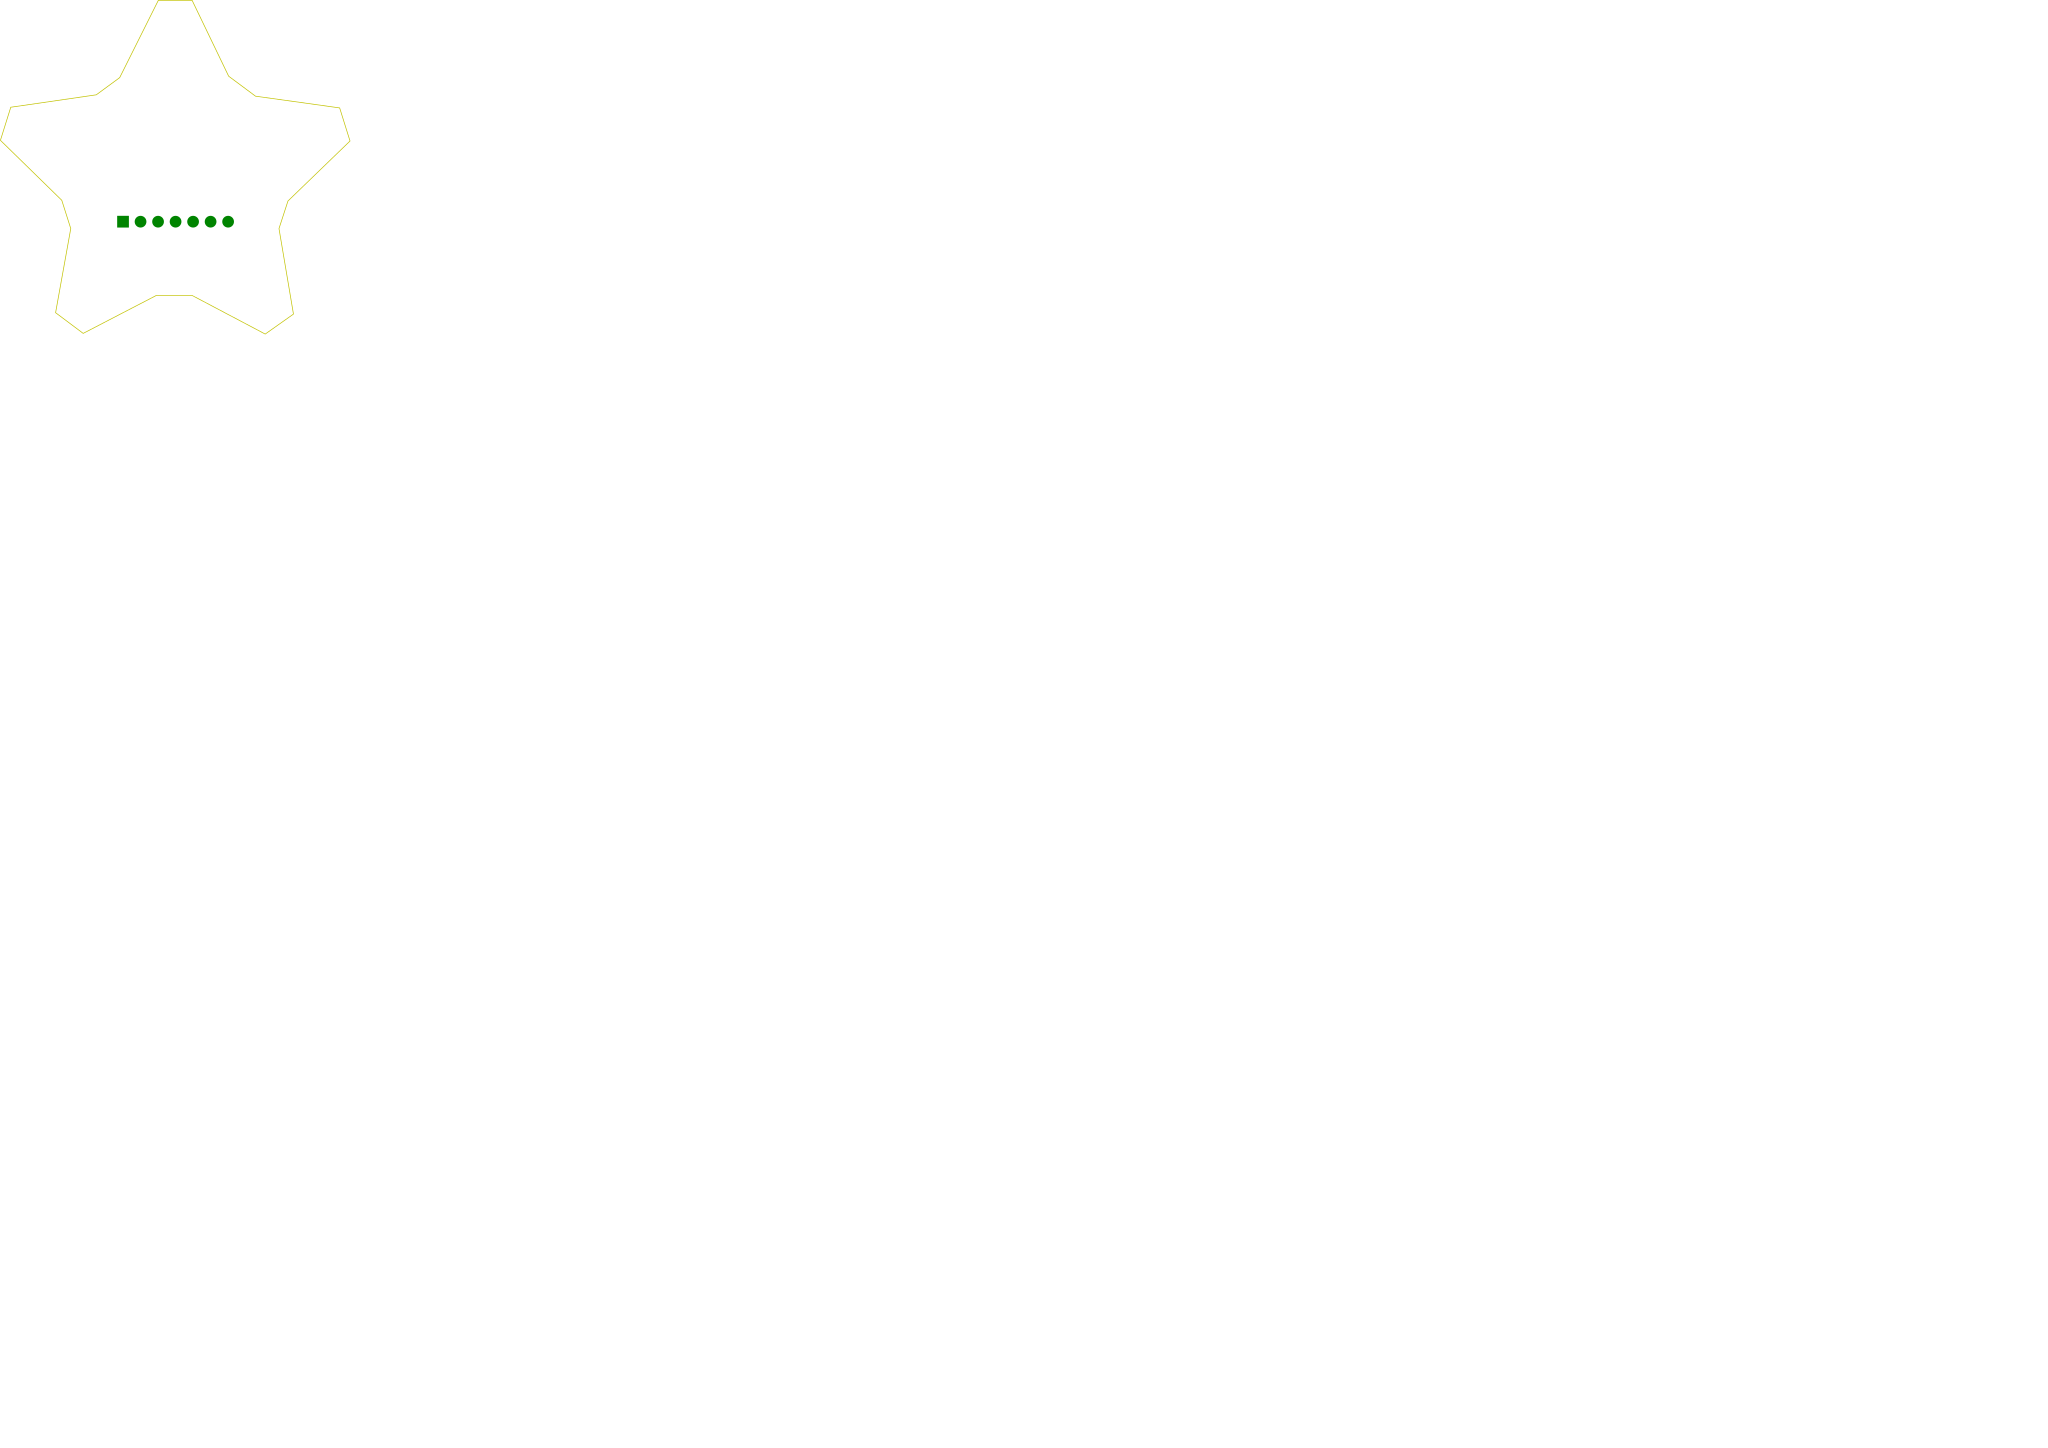
\includegraphics[width=\textwidth]{../images/manual/star-brd.pdf} % uncomment when printing in black and white
\end{figure}

\section{Introduction}

Hey there! \\
Thank you for buying this christmas kit! We (the klushok committee) hope you will enjoy building and displaying this christmas star!

\noindent The project you're about to get started on was designed by the klushok committee. It is intended to be used as a gadget and makes use of existing open source firmware. This firmware will be discussed in more detail in section \ref{sec:firmware}.\vspace{1ex}

\noindent This manual will guide you through the required steps required to assemble your star and get it up and running.
Before you get started, ensure you've received a complete kit. The required components can be found in figure \ref{fig:kitContent}, these are not drawn to scale so keep this in mind when verifying the contents of your kit. You will additionaly  need the PCB (Printed cuircuit board) shown on the cover of this manual.
When you've verified the contents of your kit, proceed to the next section.

\begin{figure}[H]
	\centering
	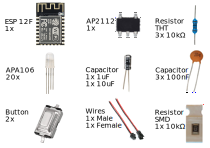
\includegraphics[width=\textwidth]{../images/manual/partList.pdf}
	\caption{Components included in the kit}
	\label{fig:kitContent}
\end{figure}
% TODO add usb breakout

\clearpage

\section{Assembly}

To assemble the star, you'll need to be familiar with soldering. Although most components are THT (through hole technology), there are some SMD (surface mount devices):
\begin{itemize}
	\item The ESP12F
	\item The reset and program buttons
	\item The LDO (low dropout) voltage regulator
	\item A pulldown resistor between GPIO15 and GND
\end{itemize}

\noindent Soldering these components requires a good pair of tweezers so make sure you have those nearby.

\subsection{Prefered order}
The prefered order is based on how easy solder pads are to access after other components have been soldered in place.
It highly depends on personal preference and since this order does not influence functionallity of the star, feel free to chose your own order.
\begin{enumerate}
	\item ESP 12F
	\item The SMD resistor between GPIO15 and GND
	\item The AP2112-3.3V LDO
	\item The THT resistors and C1 C2 and C3
	\item Optionally (see subsection \ref{subsec:optionalComponents}) C4, C5 and the SMD buttons
	\item Solder all the APA106 in place
	\item Finally solder the male connector to the GND and 5V pins.\vspace{1ex}\\ \textit{\textbf{Hint}: If you don't plan on adding an additional string to the hole just above the GND and 5V pads, put the red wire through the hole before soldering it to the 5V pad. This will decrease the strain on the solder joint and reduce the chance of the wires breaking due to fatigue.}
\end{enumerate}

\subsection{Optional components}
\label{subsec:optionalComponents}
Not all components shown in figure \ref{fig:kitContent} are required: C4, C5 and the push buttons can be left out and the board will still function correctly. These buttons are connected to the reset and GPIO0. Both the reset and GPIO have to be pulled high for normal operation but can be pulled low for additional functionallity:
% TODO further explain what 'pulled high', 'pulled low' and 'flashing' means

\noindent If the reset button is pressed, the ESP12F will be reset. The same effect can be achieved by turning the star off and on, which is why the button and associated capacitor are optional.

\noindent GPIO0 has to be pulled high when the ESP12F starts to boot from flash instead of programming mode. The button attached to this GPIO is required if you want to reprogram the ESP12F using just the RX and TX pads.
After the ESP12F has booted, this button can be used as a regular input and could, for example, be used to toggle the star on or off or apply a different preset (see section \ref{sec:firmware}).

\noindent Both the reset and GPIO0 are used when flashing the ESP12F, which is why they're broken out.
When using the programmer supplied at the klushok, neither of these buttons is required to reprogram the star.


\subsection{Component orientation}
The orientation in which the resistors, buttons and ceramic capacitors can be soldered does not matter. This orientation does however matter for the electrolytic capacitors, the AP2112 voltage regulator, the wires, the ESP 12F and the LED's. The placement of the LED's will be discussed in detail in the subsection \ref{subsec:ledOrientation}.
\vspace{2ex}

\noindent The orientation of the electrolytic capacitors is easy: the white stripe on the black cylinder should match the white pad on the pcb.

\noindent The orientation of the ESP 12F and the AP2112 voltage regulator are self explainatory: the pads should match. For the ESP this means that the gold zigzag pattern (this is the wifi antenna) should overlap the darker green part of the PCB. The AP2112 has 3 legs on one side and 2 on the other, the two leg side should point towards the label 'U2' on the PCB.


\subsection{LED orientation}
All but one of the 20 LEDs are soldered using the pads with holes in them. \textbf{When inserting the LEDs into these holes make sure to verify the orientation!} If you solder the led in a reversed orientation, it will break once you turn on the power supply. Figure \ref{fig:ledOrientation} shows the easiest way to deduct the orientation of the LEDs: The two longer legs should go to the square solder pad and its direct neighbour.

\label{subsec:ledOrientation}
\begin{figure}[H]
	\centering
	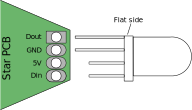
\includegraphics[width=\textwidth]{../images/manual/led_orientation.pdf}
	\caption{The square solder pad indicates where the data\_out pin of the LED should go}
	\label{fig:ledOrientation}
\end{figure}

\noindent After the LED has been put in its place, you can bend the LED to point away from the PCB as shown in figure \ref{fig:ledBent}. \\


\noindent The LED marked with label 'D12' has to be soldered without the use of any holes. The orientation is the same as shown in figure \ref{fig:ledOrientation}: the square pad indicates the Data\_out pin. The easiest way to solder this LED is to first cut the legs to size, then apply solder to 1 pad. Verify the orientation of the LED using its flat size and then solder the first leg onto the applied solder blob. The location of the LED can at this point easily be adjusted by melting this one blob and moving the LED around.

\noindent Once every leg matches its pad, apply solder to all of them to firmly attach the LED.

\vspace{1ex}
\noindent \textit{\textbf{Warning:} LED D12 is attached using surface pads only, don't try to bend this LED or you might rip the pads from the PCB!}

\begin{figure}[H]
	\centering
	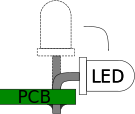
\includegraphics[width=0.5\textwidth]{../images/manual/led_bent.pdf}
	\caption{}
	\label{fig:ledBent}
\end{figure}

\subsection{Verification}
Now that every component has been soldered in place, the connections have to be checked.
This is a very important step since the ground and 5V pins are very close to each other in the footprint for the APA106.
If these pins are accidentally connected, this will short the power supply.
The easiest way to check this is by using the continuity setting on your digital multimeter and measuring the resistance across the 5V and GND pins.\\

\vspace{1ex}
\textit{\textbf{Note:} When measuring continuity across a capacitor, a continuity will be measured for a short period of time. This is due to the charging of the capacitors and is expected (and thus correct) behaviour.}

\subsection{Power source}
To connect the star to the power supply, a mini-USB breakout has been added to each kit. This breakout allows you to connect one or multiple stars to the same power supply using a regular USB A to mini USB cable. The other side of the wire you soldered to the GND and 5V pads in the previous steps can be connected to the GND and VBUS pins of the breakout respectively.



\section{Firmware}
\label{sec:firmware}
The recommended firmware for this project is an open source firmware project called WLED\footnote{https://github.com/Aircoookie/WLED}. WLED contains many options and built-in effects in addition to integrations into popular programms like Home Assistant. Control of a WLED device can be done using the web interface or the app available for both IOS and Android.\\\hfill

\noindent This section will shortly discuss the required configurations to get the star running, provided WLED has already been flashed to the ESP 12F. Kits bought during Christmas 2021 will have their firmware flashed before being sold.

Since development of WLED is ongoing, any information provided in this section can be depracated. This manual is written for firmware version 0.12.0.
A more detailed and up to date description of WLED can be found on its website: \url{https://kno.wled.ge/}. Newer versions can easily be installed using the WLED web installer: \url{https://install.wled.me/}.

\subsection{Inital connection}
When a WLED device can't connect to a known network, it will deploy its own wifi network. By connecting to this network the device can either be controlled directly or be configured to connect to an existing wifi network.
The default network name is "WLED-AP" with password "wled1234".


\subsection{Configuration}
The star contains a total of 20 LEDs. This must be entered at the top of the "LED \& Hardware setup" config page. Although these are APA106 LEDs, the LED type must be set to "WS281X" with color order "RGB".
Figure \ref{fig:wledConfig} shows the correct settings The maximum current setting is up to you and depends on the 5V source you used. The warning to keep the maximum current below 1A can safely be ignored.

\begin{figure}[H]
	\centering
	\includegraphics[width=0.5\textwidth]{../images/manual/wled_config.png}
	\caption{}
	\label{fig:wledConfig}
\end{figure}

\clearpage
\appendix
\includepdf[fitpaper=true,pagecommand={\thispagestyle{importedpages}}]{../images/manual/schematic.pdf}

\end{document}


